% MLI schedule figure for the README (same drawing as the poster's "Attend the previous indexer's selection" block).
% Build: pdflatex fig_mli_schedule.tex, then crop/render to PNG.
\documentclass{article}
\usepackage[paperwidth=20cm,paperheight=8cm,margin=0.5cm]{geometry}
\pagestyle{empty}\setlength{\parindent}{0pt}
\usepackage[T1]{fontenc}
\usepackage[sfdefault,book,lining]{FiraSans}
\usepackage{newtxsf}
\usepackage{amsmath}
\usepackage{xcolor}
\usepackage{tikz}
\usetikzlibrary{arrows.meta}
\definecolor{inksec}{HTML}{52514E}\definecolor{muted}{HTML}{898781}
\definecolor{navy}{HTML}{0D366B}\definecolor{mli}{HTML}{2A78D6}\definecolor{mliwash}{HTML}{E6F0FC}
\definecolor{idx}{HTML}{EB6834}\definecolor{attn}{HTML}{1BAF7A}
\begin{document}
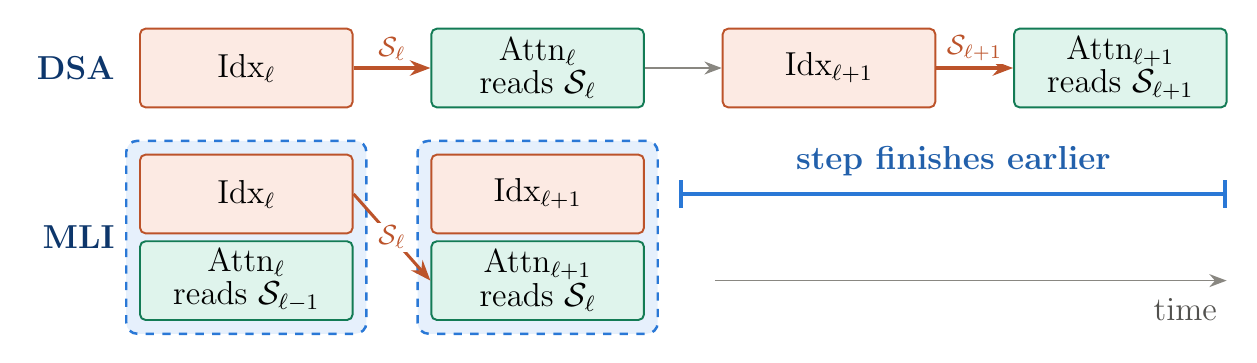
\begin{tikzpicture}[x=1cm,y=1cm,font=\large,
  bx/.style={line width=0.7pt,rounded corners=2pt,minimum width=2.7cm,minimum height=1.0cm,inner sep=1pt,align=center},
  ix/.style={bx,draw=idx!80!black,fill=idx!14},
  atn/.style={bx,draw=attn!70!black,fill=attn!14},
  stp/.style={draw=mli,dashed,line width=0.9pt,rounded corners=4pt,fill=mliwash,minimum width=3.05cm,minimum height=2.45cm},
  sel/.style={-{Stealth[length=2.6mm]},line width=1.1pt,idx!80!black},
  dep/.style={-{Stealth[length=2.2mm]},line width=0.7pt,muted},
  lab/.style={font=\normalsize,fill=white,inner sep=1pt},
  ttl/.style={font=\large\bfseries,text=navy,anchor=east,align=right}]
% ---- standard DSA: every attention waits for its own indexer
\node[ttl] at (-0.2,3.45) {DSA};
\node[ix]  (L1) at (1.35,3.45)  {Idx$_\ell$};
\node[atn] (L2) at (5.05,3.45)  {Attn$_\ell$\\[-2pt]reads $\mathcal{S}_\ell$};
\node[ix]  (L3) at (8.75,3.45)  {Idx$_{\ell+1}$};
\node[atn] (L4) at (12.45,3.45) {Attn$_{\ell+1}$\\[-2pt]reads $\mathcal{S}_{\ell+1}$};
\draw[sel] (L1) -- node[lab,above=1pt]{$\mathcal{S}_\ell$} (L2);
\draw[dep] (L2) -- (L3);
\draw[sel] (L3) -- node[lab,above=1pt]{$\mathcal{S}_{\ell+1}$} (L4);
% ---- MLI: a layer's indexer and attention share one step
\node[ttl] at (-0.2,1.3) {MLI};
\node[stp] at (1.35,1.3) {};
\node[stp] at (5.05,1.3) {};
\node[ix]  (R1) at (1.35,1.85) {Idx$_\ell$};
\node[atn] (R2) at (1.35,0.75) {Attn$_\ell$\\[-2pt]reads $\mathcal{S}_{\ell-1}$};
\node[ix]  (R3) at (5.05,1.85) {Idx$_{\ell+1}$};
\node[atn] (R4) at (5.05,0.75) {Attn$_{\ell+1}$\\[-2pt]reads $\mathcal{S}_\ell$};
\draw[sel] (R1.east) -- node[lab,pos=0.5]{$\mathcal{S}_\ell$} (R4.west);
\draw[mli,line width=1.3pt,{Bar[width=3.5mm]}-{Bar[width=3.5mm]}] (6.85,1.85) -- (13.8,1.85);
\node[text=mli!80!black,font=\large\bfseries,anchor=south] at (10.33,1.95) {step finishes earlier};
\draw[-{Stealth[length=2.2mm]},muted,line width=0.6pt] (7.3,0.75) -- (13.8,0.75);
\node[text=inksec,anchor=north east] at (13.8,0.65) {time};
\end{tikzpicture}
\end{document}
